\documentclass[varwidth,convert={density=500,size=1080x800,outext=.png}]{standalone}
\usepackage{mathtools}
\usepackage{graphicx}
\usepackage{bm}
\usepackage{color}
\usepackage[dvipsnames,table]{xcolor}
\usepackage{tikz}
\usepackage{stanli}
\usepackage{verbatim}
\usepackage{tikz}
\usetikzlibrary{shapes,calc,through,3d,patterns}
\usetikzlibrary{decorations.pathreplacing}
\usepackage{pgfplots}
\usepackage{siunitx} % For formatting numbers
\usepackage{hyperref}
\hypersetup{colorlinks=true,linkcolor=darkred}
\usepackage{multicol}
\usepackage[absolute,overlay,]{textpos}
\usepackage{pgfplots}
\pgfplotsset{width=10cm,compat=1.9}
\usepackage{subcaption}
\usepackage{multirow}
\usepackage{bbding}
\usepackage{arydshln}
\usepackage{mathtools}
\usepackage{tcolorbox}

\usepackage[dvipsnames]{xcolor}

\definecolor{darkred}{rgb}{0.6,0,0}

\begin{document}
      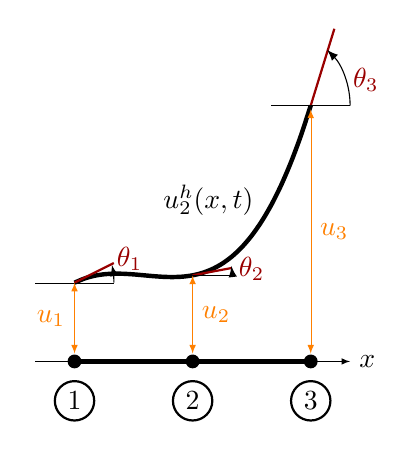
\begin{tikzpicture}[scale=1]
        % Define points
        \coordinate (A) at (0, 0);
        \coordinate (B) at (3, 0);
        \coordinate (M) at (1.5, 0);
        % Mark points
        \fill (A) circle (2.5pt);
        \fill (B) circle (2.5pt);
       \fill (M) circle (2.5pt);
               % Label the element
        \draw[ultra thick] (A) --(B);
        \draw[thick] (A) ++ (0,-0.5) circle(0.25cm) node {1};
        \draw[thick] (M) ++ (0,-0.5)  circle(0.25cm) node {2};
        \draw[thick] (B) ++ (0,-0.5)  circle(0.25cm) node {3};
        %Axis 
        \draw[-latex,ultra thin] (-0.5,0) --(3.5,0) node[right]{$x$};
        %Draw function
        \draw[ultra thick,domain=0:3, smooth, variable=\x]
        plot ({\x}, {(1+0.5*\x-2*\x*\x/3+1*\x*\x*\x/4)});
        \draw[thick,darkred,domain=0:0.5, smooth, variable=\x]
        plot ({\x}, {(1+0.5*\x)});
        \draw[thick,darkred,domain=3:3.3, smooth, variable=\x]
        plot ({\x}, {(3.25*\x-6.5)});
        \node[above=1pt] at (1.7, 1.7) {$u_2^h(x,t)$};
        \node[darkred, above=1pt] at (0.7, 1) {$\theta_1$};
        
                \draw[thick,darkred,domain=1.5:2, smooth, variable=\x]
        plot ({\x}, {(0.8125+ 0.1875*\x)});
        
   
        
                \draw[-latex] (2,1.09) arc (0:7:1) ;
        \node[darkred, above] at (2.25, 0.9) {$\theta_2$};
        
        
        \draw[-latex] (0.5,1) arc (0:13:1) ;
        \node[darkred, above] at (3.7, 3.3) {$\theta_3$};
        \draw[-latex] (3.5,3.25) arc (0:45:1) ;
        \draw[ultra thin] (-0.5,1) -- (0.5,1);
        \draw[ultra thin] (0.5,1.09) -- (2,1.09);
        \draw[ultra thin] (2.5,3.25) -- (3.5,3.25);
        \draw[ultra thin, orange, latex-latex] (0,1) -- (0,0.1) node[midway, left] {$u_1$};
        \draw[ultra thin, orange, latex-latex] (1.5,1.09) -- (1.5,0.1) node[midway, right] {$u_2$};
        \draw[ultra thin, orange, latex-latex] (3,3.2) -- (3,0.1) node[midway, right] {$u_3$};
      \end{tikzpicture}
  \end{document}